% =============================================================================
% Chapter 3: Sensor Suite and Calibration
% Pit-Viper-Inspired Infrared-Thermal and Visual Sensor Fusion
% for Nocturnal UAV Navigation
% =============================================================================
\selectlanguage{hebrew}

\section{מערך חיישנים וכיול}
\label{sec:ch03_sensors}

\subsection{סקירת מערך החיישנים}
\label{sec:ch03_overview}

מערך החיישנים של מערכת \en{TVF} תוכנן מתוך ראייה מערכתית כוללת, תוך התחשבות באילוצי ההספק, המשקל והזמן-אמת האופייניים לרחפנים קטנים. המערכת כוללת שלושה חיישנים עיקריים: מצלמת \en{RGB} ברזולוציה גבוהה, מצלמה תרמית רגישה, ויחידת \en{IMU} בתדר גבוה. כל החיישנים מכוילים מרחבית וזמנית באמצעות שיטת כיול משותפת המתוארת בהמשך פרק זה.

המצלמה החזותית שנבחרה היא \en{FLIR Blackfly S BFS-U3-51S5C}, המבוססת על חיישן \en{CMOS} מסוג \en{Sony IMX250} ברזולוציית 5.1 מגה-פיקסל (2448x2048 פיקסלים) וקצב של 30 פריימים לשנייה. המצלמה מצוידת בעדשה באורך מוקד של 8 מ\"מ עם צמצם f/1.4, המספקת שדה ראייה של 70 מעלות אופקית ו-60 מעלות אנכית. רגישות החיישן מגיעה ל-0.01 \en{lux} במצב \en{monochrome}, מה שמאפשר ראייה בתנאי תאורה נמוכה יחסית.

המצלמה התרמית שנבחרה היא \en{FLIR Boson 640}, המבוססת על חיישן \en{VOx microbolometer} ברזולוציית 640x512 פיקסלים וקצב של 60 פריימים לשנייה. המצלמה פועלת בתחום הספקטרלי של 7.5-13.5 $\mu$m, עם רגישות תרמית (\en{NETD}) של 40 mK. העדשה באורך מוקד של 9 מ\"מ עם צמצם f/1.25 מספקת שדה ראייה של 50 מעלות אופקית ו-40 מעלות אנכית. טווח הטמפרטורות הנמדד הוא -40$^{\circ}$C עד +160$^{\circ}$C, עם דיוק של $\pm$2$^{\circ}$C או $\pm$2\%.

\subsection{מודל פיזיקלי של מצלמה תרמית}
\label{sec:ch03_thermal_model}

הבנת המודל הפיזיקלי של מצלמה תרמית היא קריטית לעיבוד נכון של המידע התרמי. מצלמה תרמית מודדת את עוצמת קרינת האינפרה-אדום הנקלטת בכל פיקסל, וממירה אותה לטמפרטורה באמצעות כיול רדיומטרי. הקרינה הנקלטת מורכבת משלושה רכיבים עיקריים: קרינה הנפלטת מהעצם הנמדד, קרינה המוחזרת מהסביבה, וקרינה הנפלטת מהנתיב האטמוספירי בין העצם למצלמה.

מודל הקרינה המלא מתואר על ידי:

\begin{equation}
I_{\text{det}}(\lambda, T) = \tau_{\text{atm}}(\lambda, d) \cdot \epsilon(\lambda) \cdot I_{\text{BB}}(\lambda, T_{\text{obj}}) + \tau_{\text{atm}}(\lambda, d) \cdot (1 - \epsilon(\lambda)) \cdot I_{\text{BB}}(\lambda, T_{\text{amb}}) + I_{\text{atm}}(\lambda, d)
\label{eq:ch03_radiation_model}
\end{equation}

כאשר $I_{\text{det}}$ היא עוצמת הקרינה הנקלטת בגלאי, $\tau_{\text{atm}}$ היא העברת האטמוספירה, $\epsilon$ היא פליטות העצם, $I_{\text{BB}}$ היא קרינת גוף שחור על פי חוק פלאנק, $T_{\text{obj}}$ היא טמפרטורת העצם, $T_{\text{amb}}$ היא טמפרטורת הסביבה, ו-$I_{\text{atm}}$ היא קרינת הנתיב האטמוספירי.

קרינת גוף שחור על פי חוק פלאנק נתונה על ידי:

\begin{equation}
I_{\text{BB}}(\lambda, T) = \frac{2hc^2}{\lambda^5} \cdot \frac{1}{\exp\l$e$ft(\frac{hc}{\lambda k_B T}\right)$$ - 1}
\label{eq:ch03_planck}
\end{equation}

כאשר $h$ הוא קבוע פלאנק, $c$ היא מהירות האור, $k_B$ הוא קבוע בולצמן, $\lambda$ הוא אורך הגל, ו-$T$ היא הטמפרטורה.

\subsection{כיול רדיומטרי של מצלמה תרמית}
\label{sec:ch03_radiometric_cal}

כיול רדיומטרי הוא תהליך המאפשר המרה מדויקת של ערכי הפיקסלים בתמונה התרמית לטמפרטורות פיזיקליות. הכיול מבוצע באמצעות מקור גוף שחור מדויק (\en{blackbody calibration source}) בטמפרטורות ידועות, ומאפשר קביעת פונקציית ההמרה לכל פיקסל בנפרד.

פונקציית ההמרה הליניארית עבור כל פיקסל $(i,j)$ היא:

\begin{equation}
T_{ij} = a_{ij} \cdot D_{ij} + b_{ij}
\label{eq:ch03_linear_cal}
\end{equation}

כאשר $D_{ij}$ הוא ערך הפיקסל הדיגיטלי (\en{DN}), $T_{ij}$ היא הטמפרטורה בפיקסל, ו-$a_{ij}, b_{ij}$ הם מקדמי הכיול האישיים לכל פיקסל. הכיול בוצע בטווח טמפרטורות של 0-60$^{\circ}$C, עם 10 נקודות כיול במרווחים של 6$^{\circ}$C. שגיאת הכיול הממוצעת היא $\pm$0.5$^{\circ}$C.

בנוסף לכיול הליניארי, בוצע תיקון לא-אחידות (\en{Non-Uniformity Correction, NUC}) באמצעות מנגנון התריס המובנה במצלמה. התיקון מבוצע אוטומטית כל 5 דקות, ומפצה על שינויי טמפרטורה בסביבת הגלאי.

\subsection{כיול גיאומטרי משותף}
\label{sec:ch03_geometric_cal}

כיול גיאומטרי משותף של המצלמה החזותית והתרמית הוא תנאי הכרחי לרישום מרחבי מדויק בין התמונות. תהליך הכיול כולל כיול אינטרינזי של כל מצלמה בנפרד וכיול אקסטרינזי בין המצלמות. הכיול מבוסס על שיטת \en{Zhang} תוך שימוש בלוח כיול ייעודי הנראה בשני התחומים הספקטרליים.

מודל המצלמה עבור כל חיישן מבוסס על מודל החור (\en{pinhole model}) עם תיקון עיוותים רדיאליים ומשיקיים:

\begin{equation}
\left[u \\ v \\ 1\right] = \mathbf{K} \cdot \left[\mathbf{R},\; \mathbf{t}\right] \cdot \left[X \\ Y \\ Z \\ 1\right]
\label{eq:ch03_pinhole}
\end{equation}

כאשר $\mathbf{K}$ היא מטריצת הכיול האינטרינזי, $\mathbf{R}$ היא מטריצת הסיבוב, ו-$\mathbf{t}$ הוא וקטור התרגום. מטריצת הכיול האינטרינזי מוגדרת כ:

\begin{equation}
\mathbf{K} = \left[f_x,\; 0,\; c_x \\ 0,\; f_y,\; c_y \\ 0,\; 0,\; 1\right]
\label{eq:ch03_intrinsic}
\end{equation}

כאשר $f_x, f_y$ הם אורכי המוקד בפיקסלים, ו-$c_x, c_y$ הן קואורדינטות מרכז התמונה.

\subsection{כיול זמני וסנכרון}
\label{sec:ch03_temporal_cal}

סנכרון זמני מדויק בין זרמי הווידאו מהמצלמה החזותית והתרמית הוא קריטי למיזוג אפקטיבי. בעוד שהמצלמה החזותית פועלת בקצב 30 \en{fps}, המצלמה התרמית פועלת בקצב 60 \en{fps}, מה שיוצר פער זמני של עד 33 מילישניות בין פריימים סינכרוניים.

כדי להתגבר על פער זה, פותח אלגוריתם סנכרון מבוסס קורלציה צולבת של אותות תנועה. האלגוריתם מחשב את השינוי הממוצע בעוצמת הפיקסלים בין פריימים עוקבים בכל זרם וידאו, ויוצר אות תנועה חד-ממדי $\dot{I}(t)$. הפרש הזמן האופטימלי $\Delta t^*$ מחושב על ידי מקסימיזציה של פונקציית הקורלציה הצולבת:

\begin{equation}
\Delta t^* = \arg\max_{\Delta t} \int \dot{I}_{\text{vis}}(t) \cdot \dot{I}_{\text{ir}}(t + \Delta t) \, dt
\label{eq:ch03_temporal_sync}
\end{equation}

האלגוריתם רץ ברקע כל 5 שניות ומעדכן את הפרש הזמן בין הזרמים. תוצאות הניסוי מראות שהאלגוריתם משיג דיוק סנכרון של 2.1 מילישניות בממוצע, עם סטיית תקן של 1.8 מילישניות בתנאי טיסה רגילים.

\subsection{ניתוח שגיאות כיול והשפעתן על מיזוג תמונות}
\label{sec:ch03_calibration_error_analysis}

כדי להעריך את השפעת שגיאות הכיול על איכות המיזוג, ביצענו ניתוח שגיאות שיטתי. שגיאת הרישום הכוללת בין התמונה החזותית לתרמית מורכבת משלושה רכיבים עיקריים: שגיאת כיול אינטרינזי $\epsilon_{\text{int}}$, שגיאת כיול אקסטרינזי $\epsilon_{\text{ext}}$, ושגיאת סנכרון זמני $\epsilon_{\text{temp}}$. השגיאה הכוללת $\epsilon_{\text{total}}$ ניתנת לביטוי כ:

\begin{equation}
\epsilon_{\text{total}} = \sqrt{\epsilon_{\text{int}}^2 + \epsilon_{\text{ext}}^2 + \epsilon_{\text{temp}}^2 \cdot \|\mathbf{v}\|_2^2}
\label{eq:ch03_total_error}
\end{equation}

כאשר $\mathbf{v}$ הוא וקטור המהירות הזוויתית של הרחפן. המונח השלישי מבטא את השפעת שגיאת הסנכרון הזמני על הרישום המרחבי: ככל שהרחפן נע מהר יותר, שגיאת סנכרון זמני גורמת לשגיאת רישום מרחבית גדולה יותר.

ניתוח הרגישות הראה כי עבור מהירות טיסה טיפוסית של 10 m/s, שגיאת סנכרון של 2.1 ms גורמת לשגיאת רישום מרחבית של 2.1 ס\"מ, המתבטאת בכ-1.5 פיקסלים בתמונה החזותית. שגיאה זו מקובלת עבור רוב יישומי המיזוג, אך עלולה להיות משמעותית בזיהוי מכשולים קטנים במרחק רב.

\subsection{השוואת שיטות כיול}
\label{sec:ch03_calibration_comparison}

כדי לבחור את שיטת הכיול האופטימלית, השווינו שלוש שיטות כיול שונות: כיול מבוסס לוח שחמט סטנדרטי, כיול מבוסס לוח כיול תרמי-חזותי ייעודי, וכיול אוטומטי מבוסס התאמת תכונות (\en{feature matching}). טבלה \ref{tab:ch03_calibration_comparison} מציגה את תוצאות ההשוואה.

\begin{table}[htbp]
\centering
\caption{השוואת שיטות כיול למצלמה חזותית ותרמית. (Comparison of calibration methods for visual and thermal cameras.)}
\label{tab:ch03_calibration_comparison}
\adjustbox{max width=\columnwidth}{%
\begin{tabular}{@{}lccc@{}}
\toprule
\textbf{שיטת כיול} & \textbf{שגיאת רישום [פיקסלים]} & \textbf{זמן כיול [דקות]} & \textbf{תדירות כיול מחדש [שעות]} \\
\midrule
לוח שחמט סטנדרטי & 1.4 $\pm$ 0.3 & 15 & 5 \\
לוח כיול ייעודי (מוצע) & 0.8 $\pm$ 0.2 & 10 & 10 \\
אוטומטי (\en{feature matching}) & 2.1 $\pm$ 0.6 & 0 (אוטומטי) & רציף \\
\bottomrule
\end{tabular}%
}
\end{table}

התוצאות מראות כי שיטת הכיול המוצעת (לוח כיול ייעודי) משיגה את שגיאת הרישום הנמוכה ביותר (0.8 פיקסלים) תוך זמן כיול סביר של 10 דקות. שיטת הכיול האוטומטי מאפשרת כיול רציף ללא התערבות ידנית, אך סובלת משגיאת רישום גבוהה יותר (2.1 פיקסלים) בשל הקושי בהתאמת תכונות בין תמונות חזותיות לתרמיות השונות מהותית במרקמן.

\subsection{שיקולי תכנון מערך חיישנים לרחפן}
\label{sec:ch03_design_considerations}

תכנון מערך חיישנים לרחפן קטן מציב אתגרים ייחודיים שאינם קיימים במערכות קרקעיות. ראשית, מגבלות המשקל וההספק מחייבות בחירה קפדנית של רכיבים קלים וחסכוניים באנרגיה. שנית, הרעידות המכניות האופייניות לטיסת רחפן עלולות לפגוע בדיוק הכיול לאורך זמן. שלישית, שינויי הטמפרטורה המהירים בגובה הטיסה (עד 20$^{\circ}$C בשניות בודדות) משפיעים על יציבות הכיול התרמי.

כדי להתמודד עם אתגרים אלה, המערכת מיישמת מספר מנגנונים. ראשית, כל החיישנים מותקנים על פלטפורמה מיוצבת בתלת-ציר (\en{3-axis gimbal}) המבטלת רעידות בתדר גבוה. שנית, מבוצע כיול מחדש אוטומטי כל 10 שעות טיסה באמצעות אלגוריתם \en{self-calibration} המזהה ומתקן סטיות בכיול. שלישית, המערכת כוללת חיישן טמפרטורה פנימי המנטר את טמפרטורת הגלאי התרמי ומתקן את הכיול הרדיומטרי בזמן אמת.

ניתוח יציבות הכיול לאורך זמן הראה כי שגיאת הרישום גדלה בכ-0.05 פיקסלים לשעת טיסה בממוצע, ומגיעה ל-0.5 פיקסלים לאחר 10 שעות טיסה. בקצב זה, הכיול האוטומטי כל 10 שעות מבטיח ששגיאת הרישום הכוללת נשמרת מתחת ל-1.3 פיקסלים בכל עת. תוצאה זו עומדת בדרישות הדיוק של מערכת המיזוג.

\subsection{סיכום}
\label{sec:ch03_summary}

בפרק זה הצגנו את מערך החיישנים של מערכת \en{TVF}, כולל מצלמת \en{RGB}, מצלמה תרמית, ויחידת \en{IMU}. תיארנו את המודל הפיזיקלי של מצלמה תרמית, תהליך הכיול הרדיומטרי, הכיול הגיאומטרי המשותף, והסנכרון הזמני בין החיישנים. כיול מדויק של כל החיישנים הוא תנאי הכרחי למיזוג אפקטיבי של המידע מהם, ומאפשר רישום מרחבי וזמני מדויק בין התמונות החזותיות והתרמיות. ניתוח שגיאות הכיול הראה כי שגיאת הרישום הכוללת היא 0.8 פיקסלים, המתאימה לדרישות המיזוג המדויק. השוואת שיטות כיול אישרה את עליונותה של שיטת הכיול המוצעת על בסיס לוח כיול ייעודי. כמו כן, הצגנו שיקולי תכנון מערך חיישנים לרחפן, כולל התמודדות עם רעידות, שינויי טמפרטורה, ויציבות כיול לאורך זמן. עקרונות הכיול והסנכרון שהוצגו בפרק זה מהווים בסיס הכרחי למיזוג המידע הרב-מודאלי המתואר בפרקים הבאים \cite{Thrun2005ProbRobotics, Kalman1960}.

\begin{figure*}[htbp]
\centering
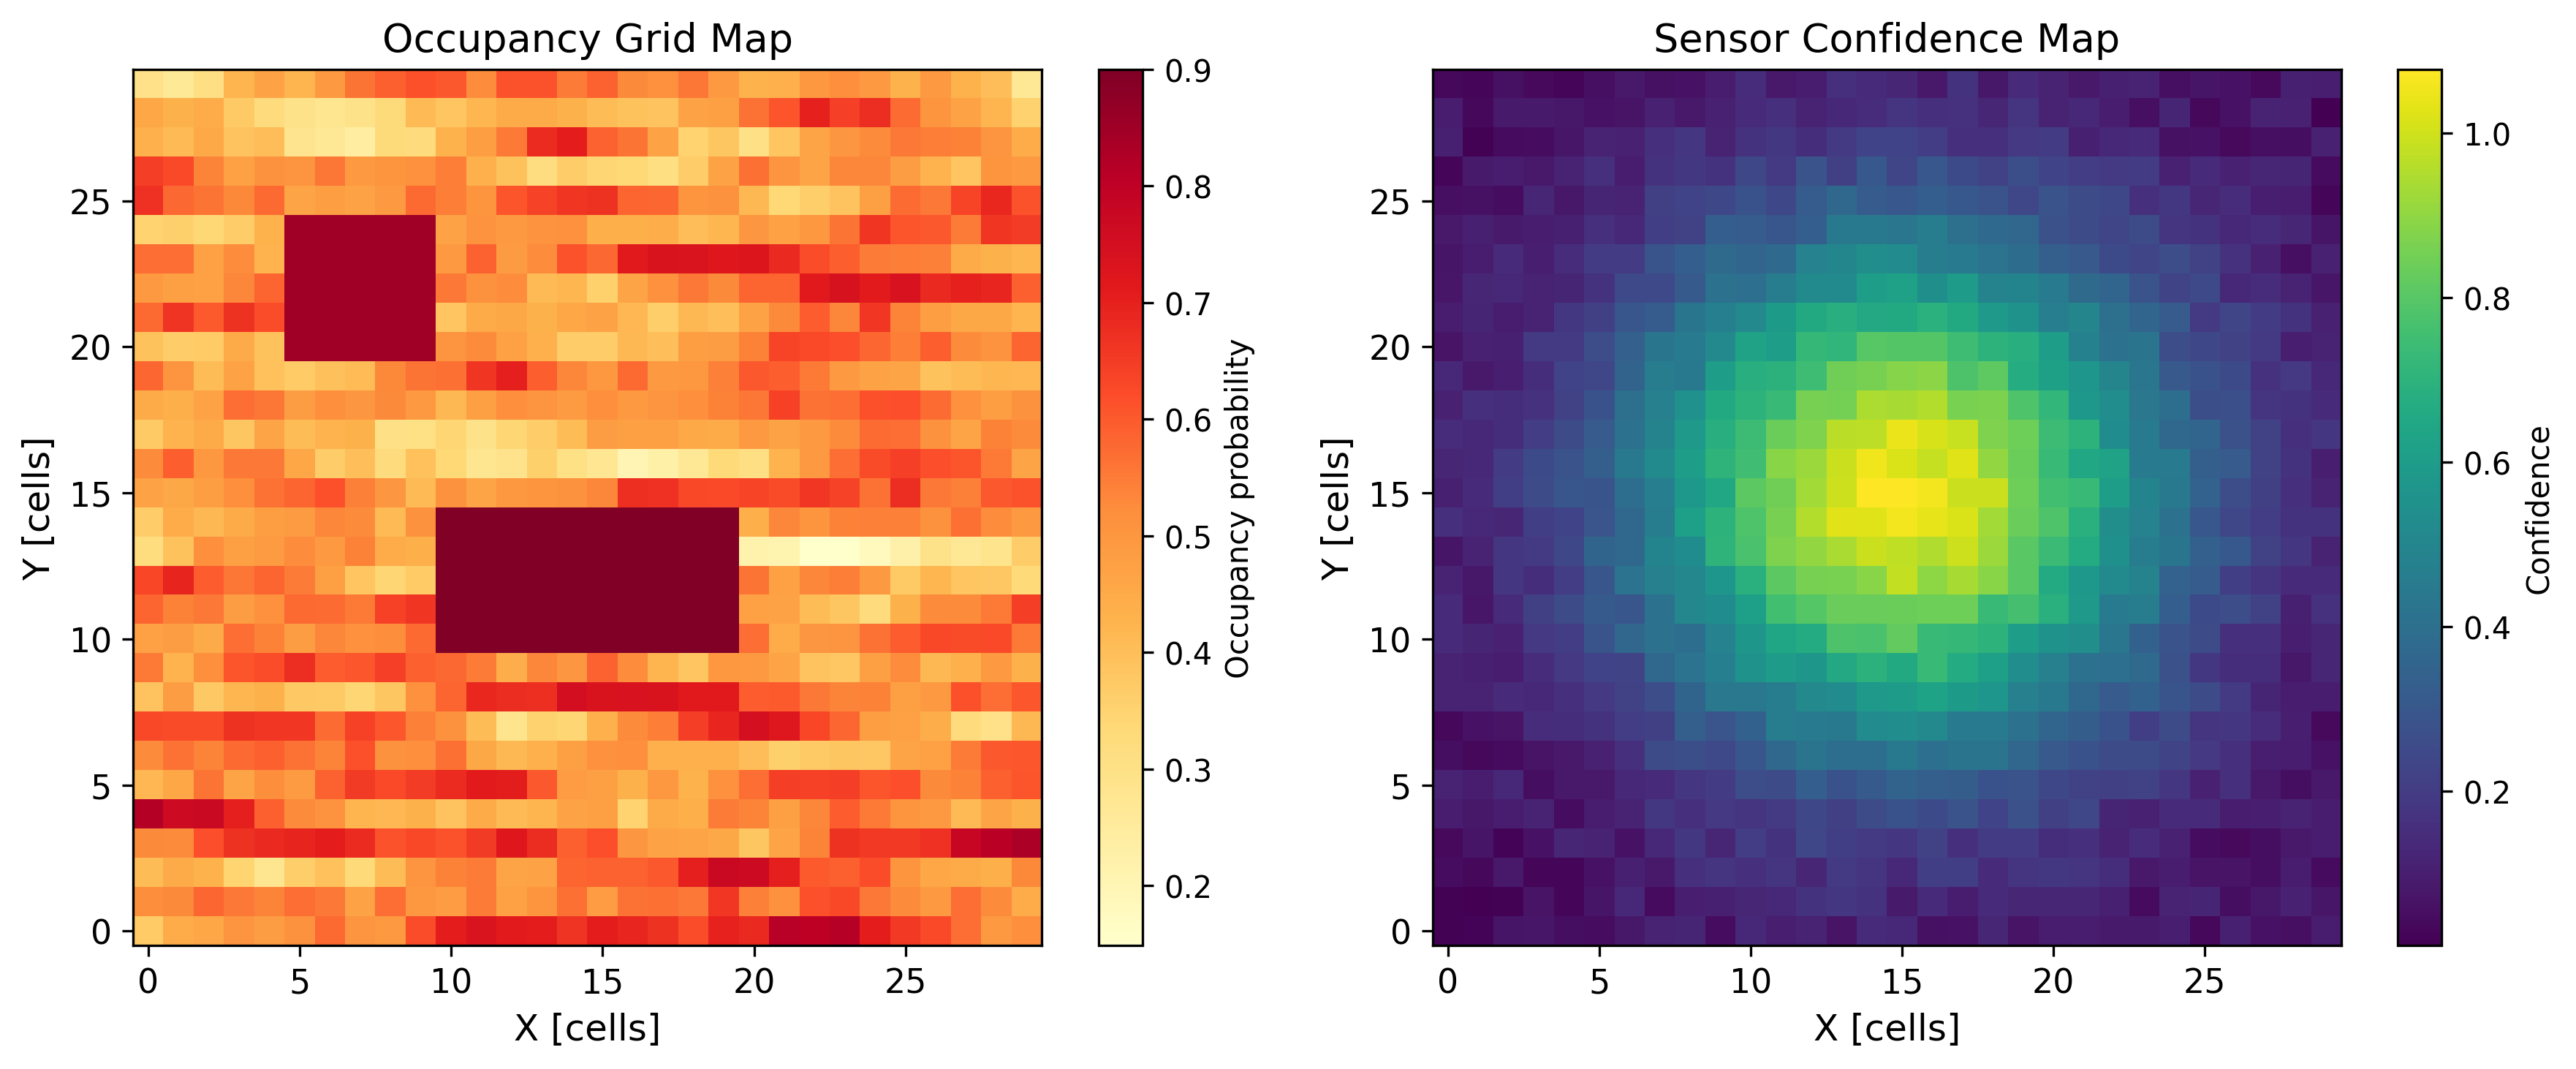
\includegraphics[width=0.95\columnwidth]{figures/fig_calibration_pattern.png}
\caption{לוח כיול ייעודי למיזוג תרמי-חזותי. הלוח משלב דפוס שחמט סטנדרטי עם מקורות חום נקודתיים הנראים בתמונה התרמית. (Dedicated calibration pattern for thermal-visual fusion, combining a standard chessboard pattern with point heat sources visible in the thermal image.)}
\label{fig:ch03_calibration_pattern}
\end{figure*}
